\definecolor{ckaVisA}{HTML}{3E6AA8}
\definecolor{ckaVisB}{HTML}{7FA8D9}
\definecolor{ckaBridge}{HTML}{D9AE3E}
\definecolor{ckaLang}{HTML}{5A9E5A}
\definecolor{ckaAct}{HTML}{C44E52}
\newcommand{\ckasw}[1]{\textcolor{#1}{\rule{4.5pt}{4.5pt}}}
\newcommand{\ckaW}{0.172\textwidth}
\newcommand{\ckahead}[1]{%
    \begin{minipage}[c]{\ckaW}\centering
        \textbf{\footnotesize #1}%
    \end{minipage}}
\newcommand{\ckaarch}[2]{%
    \begin{minipage}[c]{0.07\textwidth}\centering
        \textbf{\scriptsize #1}\\{\tiny (#2)}%
    \end{minipage}}
\newcommand{\ckacell}[1]{%
    \begin{minipage}[c]{\ckaW}\centering
        \includegraphics[width=0.97\linewidth]{images/cka_cells/#1}%
    \end{minipage}}

\begin{figure}[tp]
    \centering
    \setlength{\abovecaptionskip}{4pt}
    \setlength{\belowcaptionskip}{-8pt}
    \setlength{\tabcolsep}{1.4pt}
    \resizebox{\columnwidth}{!}{%
    \begin{minipage}[c]{0.945\textwidth}
        \centering
        \begin{tabular}{cccccc}
             &
            \ckahead{Appearance} &
            \ckahead{Spatial} &
            \ckahead{Novel Object} &
            \ckahead{Instruction} &
            \ckahead{Combined} \\[2pt]
            \ckaarch{OpenVLA-OFT}{7B} &
            \ckacell{cell_openvla_appearance.pdf} & \ckacell{cell_openvla_spatial.pdf} &
            \ckacell{cell_openvla_novel.pdf} & \ckacell{cell_openvla_instruction.pdf} &
            \ckacell{cell_openvla_combined.pdf} \\
            \ckaarch{$\pi_0$}{3.3B} &
            \ckacell{cell_pi0_appearance.pdf} & \ckacell{cell_pi0_spatial.pdf} &
            \ckacell{cell_pi0_novel.pdf} & \ckacell{cell_pi0_instruction.pdf} &
            \ckacell{cell_pi0_combined.pdf} \\
        \end{tabular}\\[3pt]
        {\scriptsize
        \ckasw{ckaVisA}\,\ckasw{ckaVisB}~vision encoders \quad
        \ckasw{ckaBridge}~cross-modal bridge \quad
        \ckasw{ckaLang}~language backbone \quad
        \ckasw{ckaAct}~action head}
    \end{minipage}%
    \begin{minipage}[c]{0.1\textwidth}
        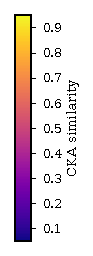
\includegraphics[width=\linewidth]{images/cka_cells/cka_colorbar.pdf}
    \end{minipage}}
    \caption{Source--target representational similarity for OpenVLA-OFT and $\pi_0$ (rows) under the five deployment shifts of Table~\ref{tab:shift-construction} (columns); the remaining three architectures appear in the accompanying video. Each matrix is linear CKA~\cite{Kornblith2019CKA} between source- and target-layer activations on \emph{paired} observations (the same LIBERO scenes rendered under both conditions), well defined across layers of different width. Role-colored bands mark the regions of Table~\ref{tab:region-partitions}. The trace beneath each matrix is the same-layer Tier~1 statistic (\S\ref{sec:method-diagnose}), the unpaired covariance-alignment score against the cached source reference that the diagnostic consumes. In each column the same role darkens across both architectures.}
    \label{fig:cka-table}
\end{figure}